\begin{figure}[t]
\centering
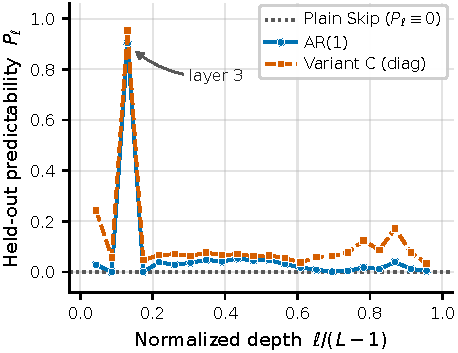
\includegraphics[width=0.62\linewidth]{figures/fig1a_predictability.pdf}
\caption{\textbf{Predictability across depth.} Held-out explained update energy $P_\ell$
against normalized depth in Qwen2.5-0.5B, for the scalar predictor (\cref{eq:ar1}) and
for \mname (\cref{eq:diag}); plain skipping is the $P_\ell \equiv 0$ baseline. The
per-channel predictor explains more of the update at nearly every depth, and layer~3
sits far above the rest at $P_\ell=0.90$, the layer that
\Cref{fig:momentum} shows is the worst of all to predict. Hardware and protocol: \Cref{sec:app-protocol}.}
\label{fig:momentum-profile}
\end{figure}
